%%%%%%%%%%%%%%%%%%%%%%%%%%%%%%%%%%%%%%%%%%%%%%%%%%%%%%%%%%%%%%%%%%%%%%%%
%                                                                      %
%     File: Thesis_Implementation.tex                                  %
%     Tex Master: Thesis.tex                                           %
%                                                                      %
%     Author: Andre C. Marta                                           %
%     Last modified :  2 Jul 2015                                      %
%                                                                      %
%%%%%%%%%%%%%%%%%%%%%%%%%%%%%%%%%%%%%%%%%%%%%%%%%%%%%%%%%%%%%%%%%%%%%%%%

\chapter{Implementation}
\label{chapter:implementation}

This section will go in depth into the implementation of the concepts presented in chapter \ref{chapter:background}. The plane model to be controlled is first implemented and verified. The first goal after this first step is to design a controller that will allow the aircraft to follow a trajectory from several position waypoints through time. The influence of certain parameters and knowledge of the exact plane model will be studied and discussed in chapter \ref{chapter:results}. The final goal will be to improve the controller and its robustness by reducing tracking error through the use of an adaptive neural network.

%%%%%%%%%%%%%%%%%%%%%%%%%%%%%%%%%%%%%%%%%%%%%%%%%%%%%%%%%%%%%%%%%%%%%%%%
\section{Plane Model}
\label{section:model}
The work made in this thesis was built on top of the work done by H. Escamilla Nuñez and  F. Mora Camino on 4D trajectory tracking \cite{hector}. The model used in this work is a six degree of freedom transport aircraft that will be described in this section. 

\subsection{Frames of Reference}
\label{section:background/model/for}
The first step before describing the dynamics of a commercial aircraft will be to define the frames of reference used to do so. The first frame of reference, on which 4D trajectories are described, corresponds to the WGS84 frame of reference. A second frame of reference corresponding to the aircraft body frame will be used to provide its fast rotational dynamics. Lastly all aerodynamic forces will be applied in the axial directions of the wind frame. This frame is aligned with the wind speed vector relative to the airplane, given by both the angle of attack $\alpha$ and the sideslip angle $\beta$. For these last two frames of reference, a rotation matrix can be defined from wind frame to body frame by


\begin{equation}
R_{BW}=
\begin{bmatrix}
c_\alpha c_\beta & -c_\alpha s_\beta & -s_\alpha \\
s_\beta & c_\beta & 0 \\
s_\alpha c_\beta & -s_\alpha s_\beta & c_\alpha
\end{bmatrix}
\label{eq:wind2body}
\end{equation}

To describe the attitude of the plane Euler, roll, pitch and yaw angles, will also be used, namely $\phi\{-\pi,\pi\}; \theta \{-\dfrac{\pi}{2},\dfrac{\pi}{2}\}; \psi \{-\pi,\pi\}$. From these angles the rotation matrix from the body to the earth frame is given by

\begin{equation}
R_{EB}=
\begin{bmatrix}
c_\theta c_\psi & s_\phi s_\theta c_\psi - c_\phi s_\psi & c_\phi s_\theta c_\psi + s_\phi s_\psi \\
c_\theta c_\psi & s_\phi s_\theta s_\psi + c_\phi c_\psi & c_\phi s_\theta s_\psi - s_\phi c_\psi \\
-s_\theta & s_\phi c_\theta & c_\phi c_\theta
\end{bmatrix}
\label{eq:body2earth}
\end{equation}

\subsection{Fast Dynamics}
\label{section:background/model/fast_dynamics}

The considered actuators of the aircraft that control its attitude are given by the control surface deflection $\delta = [\delta_{ail} \delta_{ele} \delta_{rud}]^T$, each applying a torque along an axis of the body frame. These torques are given by

\begin{equation}
\begin{bmatrix}
L'\\
M\\
N
\end{bmatrix}
= \dfrac{1}{2}\rho S V_a^2\left(
\begin{bmatrix}
bC_l\\
\bar{c}C_m\\
bC_n
\end{bmatrix}
+ C_\delta \delta\right)
\label{eq:torque}
\end{equation}

where $\bar{c}$ and $b$ represent the wing mean chord and its span respectively, $C_\delta$ and the moment coefficients $[C_l C_m C_n]^T$ are given by

\begin{equation}
C_\delta = 
\begin{bmatrix}
bC_{l\delta_{ail}} & 0 & bC_{l\delta_{rud}} \\
0 & \bar{c}C_{m\delta_{ele}} & 0 \\
bC_{n\delta_{ail}} & 0 & bC_{n\delta_{rud}}\\
\end{bmatrix}
\label{eq:cdelta}
\end{equation}
\begin{equation}
\begin{bmatrix}
C_l\\
C_m\\
C_n
\end{bmatrix} 
=
\begin{bmatrix}
C_{l\beta} \beta + C_{l_p} p \dfrac{b}{2V_a} + C_{l_r} r \dfrac{b}{2V_a}\\
C_{m_0} + C_{m_\alpha} \alpha + C_{m_q} q \dfrac{\bar{c}}{2V_a}\\
C_{n\beta} \beta + C_{n_p} p \dfrac{b}{2V_a} + C_{n_r} r \dfrac{b}{2V_a}
\end{bmatrix}
\label{eq:cmoment}
\end{equation}
Where $p, q, r$ are the body angular rates ($\Omega = [p\quad q\quad  r]^T$) and $V_a$ is the airspeed. The method for obtaining the coefficients of equation \ref{eq:cmoment} will be provided in the chapter to follow. Having defined the torques applied to the aircraft the rotational dynamics equation can now be stated as per \cite{hector}, $I$ being the aircraft inertial matrix.
\begin{subequations}
	\begin{equation}
		\dot{\Omega} = I^{-1} M_{ext} - I^{-1}\Omega \times (I\Omega)
	\end{equation}
	\begin{equation}
		\dot{\Omega} = 
		\dfrac{1}{2}\rho S I^{-1} V_a^2\left(
		\begin{bmatrix}
			bC_l\\
			\bar{c}C_m\\
			bC_n
		\end{bmatrix}
		+ C_\delta \delta\right)
		- I^{-1}\Omega \times (I\Omega)	
	\end{equation}

\label{eq:fast_dynamics}
\end{subequations}

These two equations can be rearranged to account for the effect of the wind, allowing further on to simulate the behaviour of the airplane in the presence of wind disturbances. Let $\vec{V_G} = [u \quad v \quad w]^T$ be the speed of the CG relative to the ground, $\vec{V}$ the speed of the CG relative to the air mass and $\vec{W}$ the speed of the wind relative to the ground, then as per Etkin and Reid \cite{Etkin+Reid} 
\begin{equation}
\vec{V_G} = \vec{V} + \vec{W} = 
\begin{bmatrix}
V_ac_\alpha c_\beta + V_{w_x}\\
V_as_\beta+V_{w_y}\\
V_as_\alpha c_\beta + V_{w_z}
\end{bmatrix}
\label{eq:windtriangle}
\end{equation}
and $\alpha$ and $\beta$ can be computed by 
\begin{subequations}
	\begin{equation}
		\alpha = arctan\left(\dfrac{w-V_{w_z}}{uV_{w_x}}\right)
		\label{eq:alpha}
	\end{equation}
	\begin{equation}
		\beta = arctan\left(\dfrac{v-V_{w_y}}{V_a}\right)
		\label{eq:beta}
	\end{equation}
\end{subequations}

From these three equations, differentiating \ref{eq:alpha} and \ref{eq:beta}, and from equation \ref{eq:windtriangle} and the translation dynamics equation \ref{eq:boddy_acc} comes that 

\begin{equation}
\begin{bmatrix}
\dot{\alpha}\\
\dot{\beta}\\
\dot{V_a}
\end{bmatrix}
= 
\begin{bmatrix}
H_{11} & H_{12} & H_{13}\\
H_{21} & 0 & H_{23}\\
H_{31} & H_{32} & H_{33}
\end{bmatrix}
\begin{bmatrix}
p\\
q\\
r
\end{bmatrix}
+
\begin{bmatrix}
Q_1\\
Q_2\\
Q_3
\end{bmatrix}
\label{eq:alphabetadot}
\end{equation}
Where the entries of the matrix are given by

\begin{gather*}
H_{11}=\dfrac{-V_a c_\alpha s_\beta  c_\beta - V_{w_y} c_\alpha c_\beta}{V_a(1+\tan^2\alpha)c^2_\alpha c^2_\beta}\\
H_{12}=\dfrac{V_a(c^2_\alpha c^2_\beta-s^2_\alpha c^2_\beta) + V_{w_x}c_\alpha c_\beta - V_{w_z}s_\alpha s_\beta}{V_a(1+\tan^2\alpha)c^2_\alpha c^2_\beta}\\
H_{13}=\dfrac{-V_a s_\alpha s_\beta  c_\beta - V_{w_y} s_\alpha c_\beta}{V_a(1+\tan^2\alpha)c^2_\alpha c^2_\beta}\\
H_{21}=\dfrac{V_a s_\alpha c_\beta + V_{w_z}}{V_a c_\beta}\\
H_{23}=-\dfrac{V_a c_\alpha c_\beta + V_{w_x}}{V_a c_\beta}\\
H_{31}=2 \left(-V_a s_\beta s_\alpha c_\beta - V_{w_x} s_\alpha c_\beta \right)\\
H_{32}=2\left( -V_{w_z} c_\alpha c_\beta + V_as_\alpha c_\beta s_\beta
 + V_{w_z}s_\beta + V_{w_x}s_\alpha c_\beta \right)\\
H_{33}=2\left(V_{w_y}c_\alpha c_\beta - V_{w_x}s_\beta\right)\\
Q_1=\dfrac{\left(\dfrac{1}{m}F_{za} + gc_\theta c_\phi - \dot{V}_{w_z} \right)c_\alpha c_\beta - \left(\dfrac{1}{m}(F_{xa} + T)-gs_\theta - \dot{V}_{w_x}\right)}{V_a(1+\tan^2\alpha)c^2_\alpha c^2_\beta}\\
Q_2=\dfrac{\dfrac{1}{m}F_{ya}+g c_\theta s_\phi-\dot{V}_{w_y}}{c_\beta}\\
Q_3=2 \left( \left(\dfrac{-1}{m}(F_{xa}+T) + g s_\theta - \dot{V}_{w_x} \right)c_\alpha c_\beta + \left( \dfrac{-1}{m}F_{ya} - \dot{V}_{w_y} \right)s_\beta + \left(\dfrac{-1}{m}F_{za} - \dot{V}_{w_z} \right)s_\alpha c_\beta \right)
\label{eq:Ra_dot}
\end{gather*}
The forces in the air frame $F_{xa}, F_{ya}, F_{za}$ will be further detailed in the next section on translation dynamics. 

The angular rates are also related to the Euler angles. The relationship between the Euler angles and the rotation rates is also one that will prove useful when implementing the model in a Matlab simulation, and is given by

\begin{equation}
\begin{bmatrix}
\dot{\phi}\\
\dot{\theta}\\
\dot{\psi}
\end{bmatrix}
=
\begin{bmatrix}
1 & tg_\theta s_\phi & tg_\theta c_\phi\\
0 & c_\phi & -s_\phi\\
0 & \dfrac{s_\phi}{c_\theta} & \dfrac{c_\phi}{c_\theta}
\end{bmatrix}
\begin{bmatrix}
p\\
q\\
r
\end{bmatrix}
\label{eq:euler2omega}
\end{equation}

\subsection{Translation Dynamics}
\label{section:background/model/guidance_dynamics}

This subsection focuses on the forces applied to aircraft, introducing a new actuation variable, the thrust force $T$. These forces are applied along the three axes of the wind frame, lift, drag and side force, given by
\begin{equation}
\begin{bmatrix}
D\\
Y\\
L
\end{bmatrix}
= \dfrac{1}{2} \rho SV_a^2
\begin{bmatrix}
C_D\\
C_Y\\
C_L
\end{bmatrix}
\label{eq:forces}
\end{equation}
Once again, the method used to compute these coefficients will be given in the chapter \ref{chapter:implementation} in detail. These coefficients, similarly to the moment coefficients, are functions of the angle of attack, sideslip angle and airspeed, the three most relevant variables when determining aerodynamic forces and moments. Although aerodynamic forces are usually expressed in the wind frame, as the thrust is always applied along the $x$ axis of the body frame, it is necessary to rotate the aerodynamic forces to this frame. This way the sum of the airplane forces can be obtained. 

\begin{equation}
\begin{bmatrix}
F_{xa}\\
F_{ya}\\
F_{za}
\end{bmatrix}
= R_{WB}
\begin{bmatrix}
-D\\
Y\\
-L
\end{bmatrix}
\label{eq:body_forces}
\end{equation}
From Newton's Second Law comes the aircraft acceleration

\begin{equation}
\begin{bmatrix}
\dot{u}\\
\dot{v}\\
\dot{w}
\end{bmatrix}
=
\begin{bmatrix}
\dfrac{1}{m}(F_{xa} + T) - gs_\theta +rv-qw\\
\dfrac{1}{m}F_{ya} + gc_\theta s_\phi + pw - ru\\
\dfrac{1}{m}F_{za} + gc_\theta c_\phi + qu - pv
\end{bmatrix}
\label{eq:boddy_acc}
\end{equation}

An expression in the Earth frame can also be obtained

\begin{equation}
\begin{bmatrix}
\ddot{x}_E\\
\ddot{y}_E\\
\ddot{z}_E
\end{bmatrix}
= \dfrac{1}{m} R_{BE}
\begin{bmatrix}
F_{xa}+T\\
F_{ya}\\
F_{za}
\end{bmatrix}
+
\begin{bmatrix}
0\\
0\\
g
\end{bmatrix}
\end{equation}

\subsection{Actuator Dynamics}
\label{section:background/model/actuator_dynamics}

Finally, to simulate the delay response in actuation in order to have a realistic simulation, first order systems were introduced to the actuator dynamics as per \cite{hector}. For the control surfaces $\delta_i$, given a desired $\delta_i^d$ comes

\begin{equation}
\dot{\delta_i} = \dfrac{1}{\xi_i}(\delta_i^d-\delta_i)
\label{eq:actuator_dynamics}
\end{equation}

Similarly for thrust

\begin{equation}
\dot{T} = \dfrac{1}{\xi_T}(T^d-T)
\end{equation}

$\xi_i$ and $\xi_T$ are time constants. As the responsiveness of the resultant thrust will be much slower than that of the control surfaces, $\xi_T>>\xi_i$.
The chosen commercial aircraft that will be simulated is the Boeing 737-200, an aircraft with over 30 years of service for which some information of flight parameters is readily available, such as weight, wing span and mean chord. The simulation was made in a cruise flight environment, at $200$ m/s velocity at $10000$ m above the ground. The chosen inertial matrix for this aircraft is given by
\begin{equation}
\begin{bmatrix}
1278369.56 & 0 & -135588.17\\
0 & 3781267.79 & 0\\
-135588.17 & 0 & 4877649.98
\end{bmatrix}
kg.m^2
\end{equation}
The ISA atmospheric model was used to compute the air density at any given height.
\begin{table}[H]
  \centering
  \caption{Boeing 737-2 parameters}
    \begin{tabular}{rr}
    \toprule
    Weight $m$ & $52390$ kg \\
    Wing Span $b$ & $28.35$ m \\
    Wing Area $S$ & $102.0$ m$^{2}$ \\
    Wing mean chord $\bar{c}$ & $4.35$ m \\
    Length $l$ & $30.53$ m \\
    \bottomrule
    \end{tabular}%
  \label{tab:b737_parameters}
\end{table}%

The time constants used for the actuators was $\xi_{\delta_i}=50$ms and $\xi_T=4$s for the engines.
\subsection{Airplane Parameters and Coefficients}
\label{section:model/plane_dynamics}

In order to simulate the aircraft fast dynamics, its moments must first be computed to use equation \ref{eq:fast_dynamics}. The torque caused by the actuators is modelled as equation \ref{eq:cdelta}, using
\begin{gather*}
C_{L_{\delta_{ail}}}=0.02 \quad rad^{-1}\\
C_{L_{\delta_{rud}}}=0.002 \quad rad^{-1}\\
C_{M_{\delta_{ele}}}=-0.003 \quad rad^{-1}\\
C_{N_{\delta_{ail}}}= -0.002 \quad rad^{-1}\\
C_{N_{\delta_{rud}}}= -0.07 \quad rad^{-1}
\end{gather*}
The remaining aerodynamic coefficients from equation \ref{eq:cmoment} were obtained from the work of Hector Escamilla Nuñez in \cite{hector}.

In this work, neural networks were used to interpolate data from the USAF Stability and Control Digital Data Compendium. A two layer feed forward network, with a hidden sigmoid activation function and a linear output activation function, was then trained using the gathered data with the Bayesian Regulation training algorithm \cite{hector}. Indeed as stated previously, neural networks can approximate any continuous function according to the Universal Approximation Theorem. This method is therefore optimal to accurately approximate the variation of these coefficients that mainly vary with the angle of attack $\alpha$ and airspeed $V_a$. The only exception to this method was the drag coefficient, given for this aircraft by
\begin{equation}
C_D=0.0176+0.0515 C_L^2
\label{eq:cd_cl}
\end{equation}

The sum of the moments can be computed and used to obtain the rotation rates $p$, $q$ and $r$. Equation \ref{eq:euler2omega} can also be used and integrated to obtain the Euler angles. These will also be necessary for frame of reference changes, namely from body to earth and vice-versa. The aerodynamic forces were computed from equation \ref{eq:forces} using the outputs of the neural networks. The body forces and acceleration relative to the earth frame were then obtain from equations \ref{eq:body_forces} and \ref{eq:boddy_acc}. 
The effects of the wind were also taken into account by adding the wind speed to the integration of the acceleration of the aircraft relative to the earth as per \ref{eq:windtriangle}. At this point the values of $\alpha$ and $\beta$ were also obtained for their respective equations \ref{eq:alpha} and \ref{eq:beta}. 

A simplified block diagram of the plane simulator is given by figure \ref{fig:plane_model}.
\begin{figure}[!htb]
  \centering
  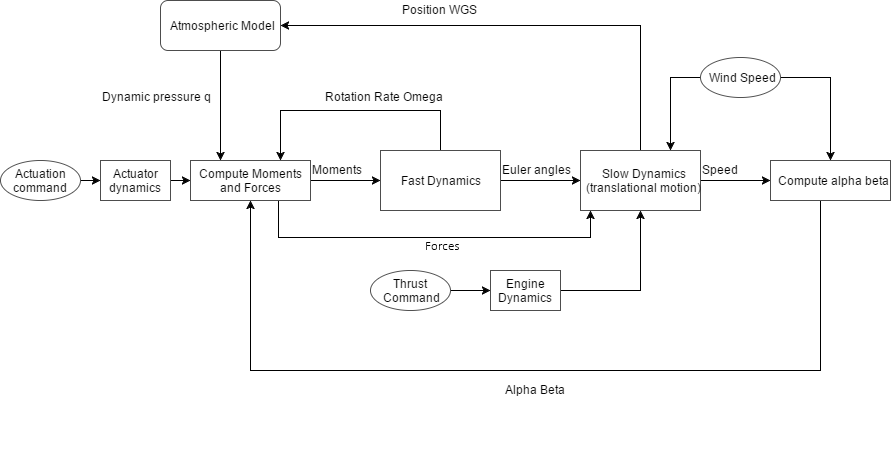
\includegraphics[width=1\textwidth]{Figures/PlaneModel.png}
  \caption[Plane dynamics simulator diagram]{Plane dynamics simulator diagram}
  \label{fig:plane_model}
\end{figure}
 

\section{Controller Implementation}
\label{section:control_implement}

To invert such a complex system (figure \ref{fig:plane_model}), two layers of inversion are proposed by H. Escamilla \cite{hector}, namely for the fast and slow dynamics. Directly controlling these are three of the four actuator control inputs, the control surfaces for the aileron, elevon and rudder. These will therefore be the output of the nonlinear inversion control. 

\subsection{Fast Dynamics}
To invert the fast dynamics equation \ref{eq:fast_dynamics} must be differentiated once, to account for both the actuator dynamics \ref{eq:actuator_dynamics} and the wind effects. Doing so yields the jerk vector given by, as per \cite{hector}

\begin{equation}
\begin{bmatrix}
\ddot{p}\\
\ddot{q}\\
\ddot{r}
\end{bmatrix}
= \dfrac{1}{2}\rho SI^{-1} \left\lbrace V_a^2 C_\delta \xi^{-1}
\begin{bmatrix}
\delta^d_{ail}-\delta_{ail}\\
\delta^d_{ele}-\delta_{ele}\\
\delta^d_{rud}-\delta_{rud}
\end{bmatrix}
+V_a^2C_c\dot{R_a}+2V_a\dot{V_a}\left(
\begin{bmatrix}
bC_l\\
\bar{c}C_m\\
bC_n
\end{bmatrix}
+ C_\delta 
\begin{bmatrix}
\delta_{ail}\\
\delta_{ele}\\
\delta_{rud}
\end{bmatrix}
\right) \right \rbrace + I^{-1}\left(\dfrac{1}{4}\rho SV_aC_k-I_n\right)\dot{\Omega}
\label{eq:jerk}
\end{equation}

where

\begin{gather*}
I=
\begin{bmatrix}
I_{xx} & 0 & -I_{xz}\\
0 & I_{yy} & 0\\
-I_{zx} & 0 & I_{zz}
\end{bmatrix}\\
I_n=
\begin{bmatrix}
-I_{xz}q & (I_{zz}-I_{yy})r-I_{xz}p & (I_{zz}-I_{yy})q\\
(I_{xx}-I_{zz})r+2I_{xz}p & 0 & (I_{xx}-I_{zz})p-2I_{xz}r\\
(I_{yy}-I_{xx})q & (I_{yy}-I_{xx})p+I_{xz}r & I_{xz}q
\end{bmatrix}\\
\xi=
\begin{bmatrix}
\xi_{ail} & 0 & 0\\
0 & \xi_{ele} & 0\\
0 & 0 & \xi_{rud}
\end{bmatrix}\\
C_c=
\begin{bmatrix}
0 & bC_{l_\beta} & -\dfrac{b^2}{2V_a^2}(C_{l_p}p+C_{l_r}r)\\
\bar{c}C_{m_\alpha} & 0 & -\dfrac{\bar{c}^2}{2V_a^2}C_{m_q}q\\
0 & bC_{n_\beta} & -\dfrac{b^2}{2V_a^2}(C_{n_p}p+C_{n_r}r)
\end{bmatrix}\\
C_k=
\begin{bmatrix}
b^2C_{l_p} & 0 & b^2C_{l_r}\\
0 & \bar{c}^2C_{m_q} & 0\\
b^2C_{n_p} & 0 & b^2C_{n_r}
\end{bmatrix}\\
\dot{Ra} =  [\dot{\alpha} \quad \dot{\beta} \quad \dot{V_a}]^T
\end{gather*}

To do a feedback linearisation, a pseudo input must be chosen, in this case $\tau = \ddot{\Omega}$. The feedback control law will therefore be, solving equation \ref{eq:jerk} for $\delta^d$,

\begin{equation}
\begin{bmatrix}
\delta^d_{ail}\\
\delta^d_{ele}\\
\delta^d_{rud}
\end{bmatrix}
=\dfrac{1}{V_a^2}\xi C_\delta^{-1}\left\lbrace\dfrac{2I}{\rho S}\tau - \dfrac{2}{\rho S}(\dfrac{1}{4}\rho S V_aC_k - I_n)\dot{\Omega} -2V_a\dot{V_a} \left(
\begin{bmatrix}
bC_l\\
\bar{c}C_m\\
bC_n
\end{bmatrix}
+ C_\delta \delta\right)-V_a^2C_c\dot{R_a} \right\rbrace+ \delta
\label{eq:control_law}
\end{equation}


Indeed, by replacing \ref{eq:control_law} in the jerk equation \ref{eq:jerk}, the equation $\ddot{\Omega} = \tau$ is obtained, resulting in a successfully inverted system.


The wind effects will appear in the terms including $\dot{R}_a =  [\dot{\alpha} \quad \dot{\beta} \quad \dot{V_a}]^T$, as the equation defining $\dot{V_a}$ can be obtained differentiating the norm of the speed relative to the ground. The value of $\dot{R}_a$ can be computed from equation \ref{eq:Ra_dot}.

Should all of the parameters mentioned in the equations above be known and no inversion error be made, the resulting system $\ddot{\Omega}=\tau$ will be both linear and decoupled, having three pseudo inputs $\tau = [\tau_p \quad \tau_q \quad \tau_r]^T$. As mentioned in section \ref{section:background/NLI}, the next step of the nonlinear inversion shall be to propose a linear controller for this resulting system. Taking the desired rotation rates $\Omega^d$ as inputs comes a control law for $\tau$, first considering without neural network adaptation
\begin{equation}
\tau = -K_P (\Omega-\Omega^d)-K_D (\dot{\Omega}-\dot{\Omega}^d)+\ddot{\Omega}^d
\label{eq:linear_controller}
\end{equation}
Where $K_P$ and $K_D$ are chosen to ensure stability and reference tracking. The previous equation can also be written as
\begin{equation}
\ddot{e}=-K_P e - K_D \dot{e}
\end{equation}
assuming that an ideal inversion is obtained and $\tau=\ddot{\Omega}$, and where $e=\Omega-\Omega^d$. 

This way the initial non-linear system becomes a second order linear one, for which natural frequencies and damping values for each dimension must be chosen. Choosing $x_1=e_i$ and $x_2=\dot{x_1}$ for a given dimension $i$ of $\Omega$, either $p,q,r$. Then comes the state equation
\begin{equation}
\begin{bmatrix}
\dot{x_1}\\
\dot{x_2}
\end{bmatrix}=
\begin{bmatrix}
0 & 1\\
-K_{P_i} & -K_{D_i}
\end{bmatrix}
\begin{bmatrix}
x_1\\
x_2
\end{bmatrix}
\end{equation}
The characteristic equation is then obtained as 
\begin{equation}
\text{det}(\lambda I-A_i)= \lambda^2 + 2\lambda\zeta_i \omega_{n_i} +  \omega_{n_i}^2 = \lambda^2 + \lambda K_{D_i} + K_{P_i} = 0
\end{equation}
\begin{gather}
\zeta_i = \dfrac{K_{D_i}\sqrt{K_{P_i}}}{2K_{P_i}}\\
\omega_{n_i}=\sqrt{K_{P_i}}
\end{gather}
The chosen values are given in table \ref{tab:tau_dynamics}.

\begin{table}[htbp]
  \centering
  \caption[Linearised system chosen dynamics]{Linearised system chosen dynamics}
    \begin{tabular}{rcccc}
    \toprule
    $i$   & $K_{P_i}$ & $K_{D_i}$ & $\zeta_i$ & $\omega_{n_i}$(rad $s^{-1}$) \\
    \midrule
    $p$   & 100   & 20    & 1     & 10 \\
    $q$   & 5     & 1     & 0.22 & 2.24 \\
    $r$   & 100   & 20    & 1     & 10 \\
    \bottomrule
    \end{tabular}%
  \label{tab:tau_dynamics}%
\end{table}%


From this point the next step will be to obtain the desired values of $\Omega$. These are obtained using another PD controller, using Euler angles values to control rotation rates. The yaw rate was set to zero as the feedback linearisation decouples the plane movement, using roll and pitch motion to turn the aircraft.

\begin{subequations}
\begin{equation}
p= k_{P_p} (\phi^d-\phi) + k_{D_p} (\dot{\phi^d}-\dot{\phi})
\end{equation}
\begin{equation}
q= k_{P_q} (\theta^d-\theta) + k_{D_q} (\dot{\theta^d}-\dot{\theta})
\end{equation}
\begin{equation}
r=0
\end{equation}
\label{eq:omega_PD}
\end{subequations}

\subsection{Slow Dynamics}

It is now possible to control the attitude of the aircraft, and the fast control loop design is completed. To follow 4D trajectories however, a guidance control loop must be designed to feed attitude and thrust reference values to the system described so far and to achieve the goal of position tracking over time. First the dynamics for speed ($V_a$), heading ($\psi$) and flight path angle ($\gamma = \theta - \alpha$) are given by, neglecting wind disturbances, from Newton's Law in the wind frame
\begin{subequations}
\begin{equation}
\dot{V_a} = \dfrac{1}{m}(T\cos \alpha -D - mg\sin \gamma)
\label{eq:va_dot}
\end{equation}
\begin{equation}
\dot{\gamma} = \dfrac{1}{mV_a}(T\sin \alpha +L - mg\cos \gamma)
\label{eq:gamma_dot}
\end{equation}
For the yaw rate comes that 

\begin{equation}
\dot{\psi} = \dfrac{g}{V_a} \tan \phi
\label{eq:psi_dot}
\end{equation}
\end{subequations}


After choosing the desired dynamics to control these variables, the equations above must be solved for both the thrust reference $T$, the desired AoA and $\psi$. From these last two, knowing the current roll angle $\theta$, the input for the fast dynamics controller is obtained. The desired dynamics were chosen as first order systems as
\begin{subequations}
\begin{equation}
\dot{V_a} = \dfrac{1}{\xi_{V_a}}(V_a^d-V_a)
\label{eq:va_dot_des}
\end{equation}
\begin{equation}
\dot{\gamma} = \dfrac{1}{\xi_{\gamma}}(\gamma^d-\gamma)
\label{eq:gamma_dot_des}
\end{equation}
\begin{equation}
\dot{\psi} = \dfrac{1}{\xi_{\psi}}(\psi^d-\psi)
\label{eq:psi_dot_des}
\end{equation}
\end{subequations}

A block diagram of the controller used to compute the pseudo input $\tau$ is described in figure \ref{fig:slow_inversion}.

\begin{figure}[!htb]
  \centering
  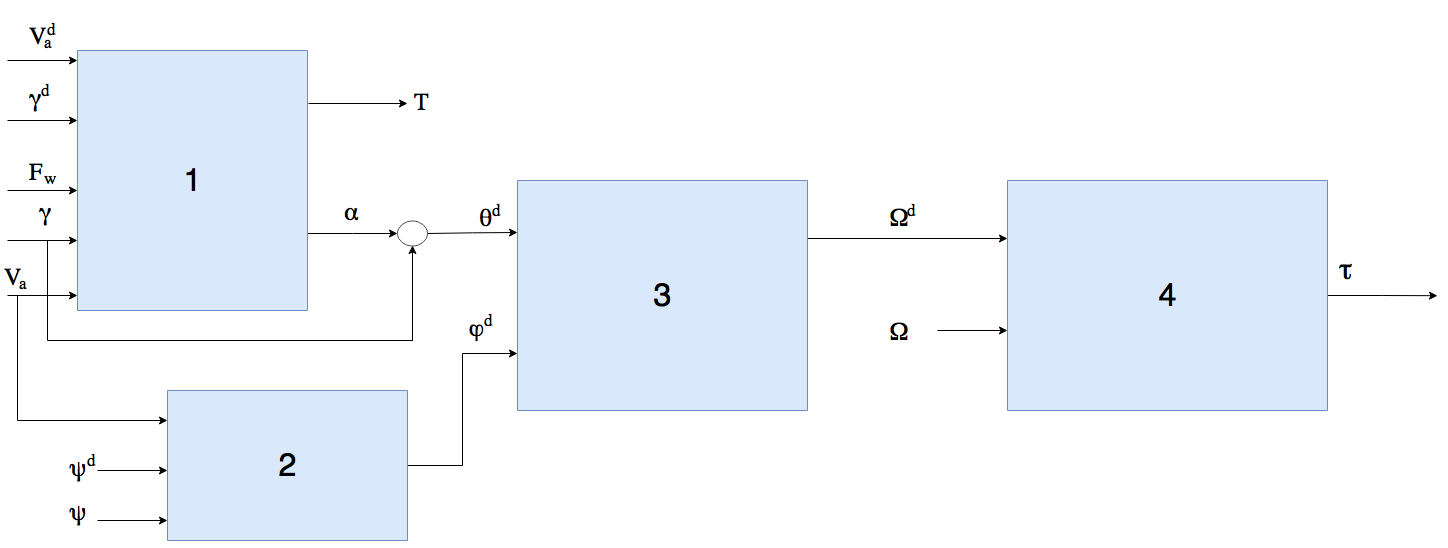
\includegraphics[width=1\textwidth]{Figures/slow_inversion.png}
  \caption[Slow dynamics controller]{This block diagram describes the method used to compute $\tau$, the pseudo input to the fast dynamics inversion. In block \textbf{1} equations \ref{eq:va_dot_des}, \ref{eq:gamma_dot_des}, \ref{eq:gamma_dot} and \ref{eq:gamma_dot} are solved to compute the desired $\theta^d$ and thrust. Similarly in block \textbf{2} equations \ref{eq:psi_dot_des} and \ref{eq:psi_dot} are also solved to obtain $\phi^d$. From these values in block \textbf{3} go through the PD controller described in equatio \ref{eq:omega_PD}, resulting in $\Omega^d$, the input of block \textbf{4}. This last block is the linear controller described by equation \ref{eq:linear_controller}, which output $\tau$.}
  \label{fig:slow_inversion}
\end{figure}

\subsection{Guidance Law}

The final step of the controller design will be to propose a guidance law to obtain the values of $V_a^d$, $\gamma^d$ and $\psi^d$ from the X,Y and Z reference values along time. For these laws it was assumed that the position reference was given relative to a frame of reference with the origin on the Earth surface, with the $Z$ axis pointing upwards. The guidance controller therefore implements the following equations, assuming the errors $\delta x = x_r - x$, $\delta y = y_r - y$ and $\delta z = z_r - z$. The $z$ formula is slightly different to the other two as in the airplane frame of reference the z axis is pointing downwards, allowing this way to use a z reference relative to the Earth surface.

\begin{subequations}
	\begin{gather}
	\delta V_a = \dfrac{1}{\tau_{V_a}}(\sqrt{\delta x^2 + \delta y^2 + \delta z^2})\\
	V_a^d= \delta V_a  + V_{a_0}
	\end{gather}
	\begin{equation}
	\psi^d = atan2(\delta y,\delta x)
	\end{equation}
	\begin{equation}
	\gamma^d = \dfrac{1}{\tau_Z}\delta z
	\end{equation}
	\label{eq:guidance_law}
\end{subequations}

This guidance law is intended to be used having at each time interval a $x_r$, $y_r$ and $z_r$ position of a desired trajectory. From these an airspeed, heading and FPA must be computed and fed to the controller. 
%TODO Paper do Hector

Taking first the airspeed equation from \ref{eq:guidance_law}, $V_{a_0}$ is the desired speed of the aircraft in cruise conditions when following the trajectory. This speed is then corrected by the term $\delta V_a$, increasing or decreasing aircraft airspeed depending on its position relative to the trajectory desired position at a given time, i.e the distance error. By dividing this error by $\tau_{V_a}$, a desired convergence time, the speed correction to the initial value $V_{a_0}$ necessary to follow a 4D trajectory is obtained. A more accurate method of obtaining an airspeed reference from these equations is specified in \ref{eq:speed_guidance}. Also, from the $x$ and $y$ position errors between the aircraft and the current trajectory waypoint the desired heading can also be computed using the $atan2$ function. Finally, the method used to obtain the Flight Path Angle relies on the error between the height of the aircraft and the desired one to compute it. 



Using solely equations \ref{eq:guidance_law} however will not grant optimal results, and may even sometimes cause loss of control of the aircraft. The goal for this 4D guidance law and of this work is to, at any given time, to be at a 3D coordinate point of a trajectory at that time. To do so, the references of speed, heading and flight path angle must be constantly adjusted to reach a 4D reference. Using the equations described previously for the guidance controller, it may happen that the aircraft would "overtake" the trajectory reference, causing the heading reference to increase to either $180^o$ or $-180^o$ and therefore making the aircraft diverge significantly from its original trajectory. To avoid this, the following guidance strategy was used:

\begin{itemize}
\item \textbf{Heading} To prevent the heading reference to excessively grow and make the aircraft do a $180^o$ turn, a small correction code in Simulink was added (see algorithm \ref{alg:psi_correction}) in order to detect large errors between the desired and measured heading, caused by the aircraft "overtaking" its trajectory. In case of large errors, this correction would force the desired heading to be equal to its measured value, thus preventing the aircraft from making large turns. 

\begin{algorithm}[H]
	\KwData{$\Psi$ and $\Psi_d$}
 \KwResult{$\Psi$ command}
 error = $\Psi_d$ - $\Psi$\;
 output = $\Psi_d$\;
 \If{$error> 160º$ or $error< -160º$}{
 output =  $\Psi$}
 
 \caption{$\Psi$ command correction algorithm}
 \label{alg:psi_correction}
\end{algorithm}


\item \textbf{Airspeed} Now that the aircraft no longer does $180^o$ turns when it overtakes the desired trajectory, the desired airspeed must be adjusted in order to slow down and therefore reach the desired position at the desired time. To do so the guidance law was slightly modified to 
\begin{equation}
V_a^d=\begin{cases}
\delta V_a  + V_{a_0} \quad \text{if} \quad |atan2(\delta y,\delta x)|<90^o\\
\delta V_a  - V_{a_0} \quad \text{if} \quad |atan2(\delta y,\delta x)|>90^o
\end{cases}
\label{eq:speed_guidance}
\end{equation}
\end{itemize}

Finally, the block diagram of the controller described thus far is given by figure \ref{fig:controller_noNN}, in which the linear controller is described in more detail in figure \ref{fig:slow_inversion}, and the plane model in figure \ref{fig:plane_model}.

\begin{figure}[!htb]
  \centering
  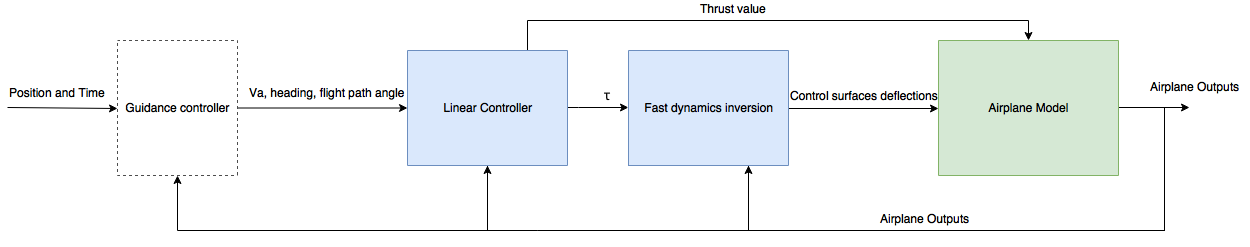
\includegraphics[width=1.15\textwidth]{Figures/controller_noNN.png}
  \caption[Diagram of the controller and model architecture, without NN compensation]{Diagram of the controller and model architecture, without NN compensation}
  \label{fig:controller_noNN}
\end{figure}

\section{Neural Network}
\label{section:NN}

Over the years, intelligent control techniques using neural networks have become a growing research topic, addressing the limitations of state-of-the-art model based controllers such as linear quadratic Gaussian, model predictive control, backstepping and gain scheduling \citep{SotA_IFCS}. Indeed, variations in the plane dynamics (e.g., due to payload changes, actuator or sensor degradation) deteriorate the error of the controller. To compensate for such errors, adaptive online neural networks have been studied and implemented in several works \cite{NLI+NN_IFCS}, \cite{NN_PID}, \cite{UAV_adaptive} and \cite{NN_NLI} to name a few. These however, have been applied almost exclusively to UAV aircraft, especially multicopters. For this work a feedforward network with one hidden layer (one of the most widely implemented neural network architecture \cite{SotA_IFCS}) was used.


\subsection{Network Architecture}
From an error-less nonlinear inversion, the pseuso-input $\tau$ would directly control $\ddot{\Omega}$ as it was seen previously. However, in case of inversion errors, that can be caused by several factors such as modelling errors or external disturbances, resulting in an equation similar to \ref{eq:system+error}, that $\tau = \ddot{\Omega}^d + \Delta$, where $\Delta = \ddot{\Omega}- \ddot{\Omega} ^d$. This method adds an adaptive component $\tau_{NN}$ to the pseudo input that will approximate the behaviour of the $\Delta$ error. The resulting control law will be given by $\tau + \tau_{NN} = \ddot{\Omega}^d + \Delta$, in which as $t \rightarrow \infty$, $\tau_{NN} \rightarrow \Delta$, thus adaptively minimizing inversion errors. To do so a simple neural network architecture was chosen: a network with a single hidden layer with therefore two sets of weights $V$ and $W$ that will need to be trained, corresponding to the input weights and the hidden layer ones. As for the activation functions for the hidden layer a sigmoid function was chosen, $sig(x)=\dfrac{1}{(1+e^{-x})}$. As the outputs must not be bound between $[0;1]$, the chosen output function was a linear one. Indeed sigmoid output functions are usually used in applications where the output must be a boolean value. A description of the chosen architecture can be found in figure \ref{fig:NN}. Different numbers of neurons were used and the results obtained will be discussed in chapter \ref{chapter:results}.

\begin{figure}[!htb]
  \centering
  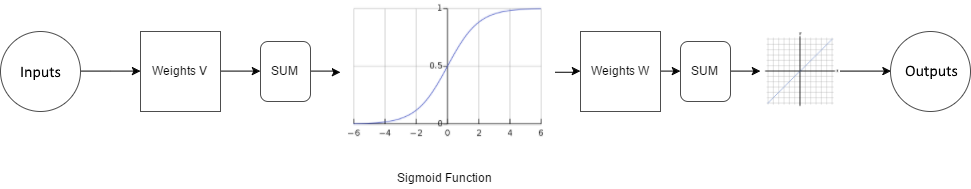
\includegraphics[width=1\textwidth]{Figures/NN.png}
  \caption[Neural Network diagram]{Neural Network diagram}
  \label{fig:NN}
\end{figure}

There are quite some challenges in designing a feed forward neural network. Besides choosing the number of layers and neurons per layer, the inputs of the network must also be chosen carefully. Some rules to choose the correct inputs are given in \cite{NN_inputs}:
\begin{itemize}
\item \textbf{Relevance}: This is the most important consideration to have while choosing inputs, this set must be sufficiently informative of the state of the system for the network to perform correctly. A NN will perform poorly if the output behaviour is not correlated to its input.
\item \textbf{Redundancy}: A large value of redundant and irrelevant input variables will not only increase the needed computational effort of the NN, but will also increase the difficulty to train the weights of the network and add noise to the system.
\end{itemize}

Another consideration about the chosen inputs that must also be taken into account is their range. The sigmoid function $sig(x)$ used reaches around 73\% when $x=1$ and 88\% when $x=2$, as can be seen in figure \ref{fig:sigmoid}. For some cases the inputs might therefore need to be normalized. While this is quite a trivial task in the case of batch training, as the minimum and maximum value of each input is easily obtained before even starting training, such is not the case for online training, and a maximum and minimum value must be proposed \emph{a priori} for each input. The mean of these values should also be close to zero. Should the input not be normalized and reach absolute values much greater than the unity, its activation function output would be constant and the system would therefore not react to input change. This, clearly, is not desirable. To map the input $x$ knowing its minimum and maximum values to its normalized equivalent $y$, the following equation is used

\begin{equation}
y=2\dfrac{x-x_{min}}{x_{max}-x_{min}}-1
\label{eq:normalisation}
\end{equation}

For this  particular case, the state variables of the fast dynamics where used as inputs of the network, namely $\Omega$ and $\dot{\Omega}$.

\begin{figure}[!htb]
  \centering
  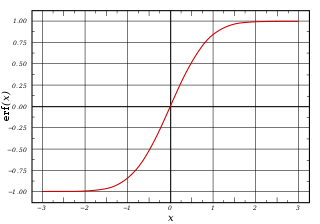
\includegraphics[width=0.5\textwidth]{Figures/sigmoid.png}
  \caption[Sigmoid Function]{Sigmoid Function}
  \label{fig:sigmoid}
\end{figure}

\subsection{Training Algorithm}

As mentioned in section \ref{section:background/NN}, a backpropagation algorithm was used to train both sets of weights online. This algorithm, however, must have an error function that will be minimized by iteratively changing the values of the weights $V$ and $W$. As seen previously, an inversion error $\Delta$ will be present, where $\tau = \ddot{\Omega}^d + \Delta$. This error must be computed for each iteration to train the network to approximate this error. The error can be expressed as $\Delta=\tau - \ddot{\Omega}^d$.
From the control law used to obtain $\tau$ (\ref{eq:linear_controller}) it comes that
\begin{equation}
\Delta = -K_P(\Omega-\Omega^d)-K_D(\dot{\Omega}-\dot{\Omega}^d)
\label{eq:inversion_error}
\end{equation}
Finally the cost function used to train the network is given by

\begin{equation}
J=\dfrac{1}{2}(\Delta-y_{NN})^2
\label{eq:NN_cost}
\end{equation}

The values of $\dot{V}$ and $\dot{W}$ must now be computed, using the gradient descent method described in section \ref{section:background/NN}. As the name suggests, the back propagation algorithm first computes the weight update values for the last layers, propagating the errors to update the previous weight set. The weights are constantly updated until the error absolute value in lesser than a given value $\Delta_{max}$, in which case these are kept constant as $\dot{V}=\dot{W}=0$. 

One of the parameters that must be tuned that has the largest impact on the performance of the network is the learning rate $\alpha$. This coefficient can also be thought of as the step size in incrementing the weight sets. Let $V^*$ and $W^*$ be the two ideal set of weights that, for a given input, result in an absolutely minimal cost function. A small value will allow the weights to converge to their ideal value, although taking many iterations to do so. A large learning rate however might converge faster, but might also overshoot and miss its optimal value. The results of the variation of this rate will be studied in chapter \ref{chapter:results}.

Finally, adding the online neural network to the baseline controller, the final control architecture is obtained. For the following chapter, the controller without the correction will be tested and compared in the same conditions to the same controller including the network. A simplified diagram of the full system, (controller, model and neural network), can be seen in figure \ref{fig:full_controller}.
\begin{figure}[!htb]  
  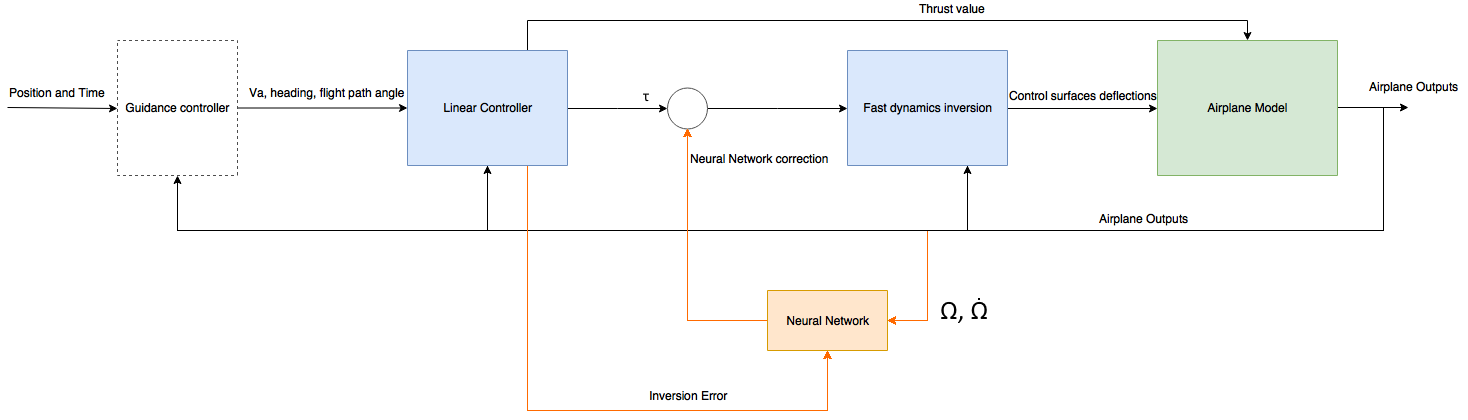
\includegraphics[width=1.1\textwidth]{Figures/full_controller_special.png}
  \caption[Diagram of the controller architecture]{Diagram of the controller architecture including NN correction (in orange)}
  \label{fig:full_controller}
\end{figure}
